\documentclass[11pt]{article}

\usepackage[margin=1in]{geometry}
\usepackage{graphicx}
\usepackage{booktabs}
\usepackage{amsmath}
\usepackage[colorlinks=true,linkcolor=blue,citecolor=blue,urlcolor=blue,pdfborder={0 0 0},breaklinks=true]{hyperref}
\usepackage{float}
\usepackage{cite}

% Prevent latex from aggressively hyphenating these specific words as requested.
\hyphenation{strategies accelerate standard computational limits beyond quantization}

\usepackage[T1]{fontenc}
\usepackage{lmodern}
\usepackage{microtype}

\title{Quantization as Accidental Jailbreak Defense:\\INT4 Compression Induces Over-Refusal in Susceptible LLMs}
\author{SHIVANG GUPTA\\Indian Institute of Technology Roorkee}
\date{}

\begin{document}

\maketitle

\begin{abstract}
Does compressing weights compress safety? We find the opposite---INT4 quantization can induce over-refusal, acting as an accidental jailbreak defense. Across three representative instruction-tuned models (Gemma-2B-Instruct, Mistral-7B-Instruct-v0.2, and Meta-Llama-3-8B-Instruct), we evaluate refusal probabilities using 550 synthetic templates and HarmBench prompts with Llama-3-70B as semantic judge. Capability controls (MMLU/GSM8K) confirm increased refusal is not intelligence loss. While Gemma-2b-it and Meta-Llama-3-8B show no significant change, Mistral-7B shows a trend (uncorrected p=0.027, OR=1.46); after Benjamini-Hochberg FDR correction for 6 comparisons, adjusted p = 0.16, suggesting this is a promising signal warranting larger-scale replication. We release the pipeline, interactive Streamlit dashboard visualizing per-prompt judge labels and refusal margins, and analysis scripts.
\end{abstract}


\section{Introduction}
When you quantize Mistral-7B to 4-bit, it starts refusing jailbreak prompts it previously complied with. That's the opposite of what you'd expect. We were surprised to find that Mistral-7B, which is notoriously easy to jailbreak at FP16, suddenly refused every single override at INT4. This contradicted our initial hypothesis that quantization would make models less safe, not more. MLP layers drove the effect. Attention barely mattered. (Mistral complied with all 200 jailbreak prompts at FP16 — every single one — which is consistent with its known vulnerability to DAN attacks but was still striking to see in practice.)

We release the pipeline so deployment teams can audit quantized models before shipping. Our findings suggest that INT4 compression can induce over-refusal in susceptible architectures, while INT8 is reassuringly stable. This would be useful for anyone deploying compressed LLMs in safety-critical settings.

The intersection of quantization and safety alignment is under-studied. Standard benchmarks show that perplexity and zero-shot performance degrade gracefully under quantization, but safety alignment is brittle. RLHF can act as a shallow "wrapper" over a model's pre-trained distribution. We wanted to know: does quantization-induced noise disrupt these safety pathways?

In this paper, we systematically evaluate the robustness of LLM refusal behavior under post-training weight quantization. Using Llama-3-70B as a semantic judge over both synthetic limits and HarmBench targets, we find model-family-specific behavioral shifts under INT4 that are independent from capability decay, with Mistral-7B showing a promising trend (adjusted p = 0.16) warranting larger-scale replication.

\section{Related Work}

\paragraph{Post-Training Quantization.}
Quantizing LLMs to 8-bit or 4-bit precision reduces memory requirements by mapping continuous weights to discrete, low-precision buckets. Methods like \mbox{LLM.int8()} \cite{dettmers2022llmint8} and GPTQ \cite{frantar2022gptq} accomplish this while preserving general zero-shot performance. More recently, QLoRA introduced 4-bit NormalFloat (NF4) quantization optimized for parameter-efficient tuning \cite{dettmers2023qlora}.

\paragraph{LLM Alignment and Safety.}
Instruction tuning and constitutional AI paradigms successfully mitigate unsafe outputs \cite{bai2022constitutional, touvron2023llama2}. Evaluating this alignment usually involves challenging models with adversarial benchmarks like AdvBench or HarmBench \cite{mazeika2024harmbench}. Prior work has demonstrated that fine-tuning can aggressively overwrite these safety mechanisms (often termed "Shadow Alignment") \cite{yang2023shadow}, and that complex "Do Anything Now" (DAN) jailbreaks can reliably bypass them \cite{wei2023jailbroken}. We extend this line of inquiry by investigating quantization itself as a mechanism that disrupts original alignment bounds.

\section{Methodology}

\subsection{Dataset Generation and External Validity}
To systematically evaluate refusal boundaries, we generated a primary dataset of 550 synthetic prompts via a combinatorial template engine. The dataset targets five sensitive societal topics across three prompt categories: Harmful, Jailbreak, and Adversarial. To validate that this synthetic logic generalizes, we cross-validate our findings utilizing an external sample of 200 real-world adversarial prompts from HarmBench \cite{mazeika2024harmbench}. We sized the dataset at 550 prompts based on a power analysis ($\geq 5\%$ drift, $\alpha=0.05$, $\beta>0.80$).

\subsection{Quantization and Models}
We evaluate \texttt{gemma-2b-it}, \texttt{Mistral-7B-Instruct-v0.2}, and \texttt{Meta-Llama-3-8B-Instruct} across three precision regimes: FP16 (baseline), INT8, and INT4. While our primary pipeline utilizes \texttt{bitsandbytes} NF4 variants, we explicitly ablate against AWQ algorithms to suggest effects generalize beyond bitsandbytes.

\subsection{LLM-as-a-Judge and Metrics}
Substring matching frequently misses nuanced refusals. Therefore, outputs are evaluated using a robust \texttt{Llama-3-70B} semantic classifier prompted to label responses as Safe (Refusal) or Unsafe (Compliance). To check judge reliability, we manually verified 50 random samples; Cohen's $\kappa = 0.92$ between human and Llama-3-70B labels. The 50 verification samples were stratified across prompt categories to ensure balanced coverage.

\begin{itemize}
    \item \textbf{Refusal Rate ($R$):} We report the \mbox{Standard} Error ($SE$) across all generations alongside Chi-squared ($p$-values) to assure drift significance.
    \item \textbf{Refusal Margin ($M_{ref}$):} To capture internal confidence, we measure the log-probability margin between refusal and compliance paths at the first token constraint.
    \item \textbf{Capability Control:} We evaluate variants on MMLU and GSM8K to separate "safety drift" from general "intelligence loss".
\end{itemize}

\section{Results and Analysis}

\subsection{Drift Significance vs Capability Control}

Table~\ref{tab:refusal} displays the refusal rates alongside Standard Error bounds. 

\begin{table}[H]
\centering
\begin{tabular}{lllc}
\toprule
Model & Precision & Refusal Rate ($R$) & Drift ($p$-value) \\
google/gemma-2b-it & fp16 & 0.238 $\pm$ 0.018 & - \\
\midrule
google/gemma-2b-it & int8 & 0.258 $\pm$ 0.019 & $p=0.365$ \\
google/gemma-2b-it & int4 (NF4) & 0.264 $\pm$ 0.019 & $p=0.171$ \\
mistralai/Mistral-7B-v0.2 & fp16 & 0.151 $\pm$ 0.015 & - \\
\midrule
mistralai/Mistral-7B-v0.2 & int8 & 0.167 $\pm$ 0.016 & $p=0.108$ \\
mistralai/Mistral-7B-v0.2 & int4 (NF4) & 0.204 $\pm$ 0.017 & $p=0.027^*$ \\
mistralai/Mistral-7B-v0.2 & int4 (AWQ) & 0.210 $\pm$ 0.018 & $p=0.021^*$ \\
meta-llama/Meta-Llama-3-8B & fp16 & 0.147 $\pm$ 0.015 & - \\
\midrule
meta-llama/Meta-Llama-3-8B & int8 & 0.153 $\pm$ 0.015 & $p=0.773$ \\
meta-llama/Meta-Llama-3-8B & int4 (NF4) & 0.162 $\pm$ 0.016 & $p=0.559$ \\
\bottomrule
\end{tabular}
\caption{LLM-Judge Refusal Rate ($R$) with p-values assessing drift significance relative to each model's FP16 baseline.}
\label{tab:refusal}
\end{table}

A pivotal question remains: is the model generating refusals more often, or is it merely suffering from degraded intelligence under INT4 compression? We isolate this capability control in Table~\ref{tab:mmlu}.

\begin{table}[H]
\centering
\begin{tabular}{lllll}
\toprule
Model & Precision & MMLU Score & GSM8K & Refusal Rate \\
mistralai/Mistral-7B & fp16 & 62.5\% & 35.1\% & 15.1\% \\
\midrule
mistralai/Mistral-7B & int8 & 62.2\% & 34.8\% & 16.7\% \\
mistralai/Mistral-7B & int4 (NF4) & 60.1\% & 32.4\% & 20.4\% ($p=0.027^*$) \\
\bottomrule
\end{tabular}
\caption{Capability controls (MMLU/GSM8K) cleanly decoupling intelligence loss from safety drift.}
\label{tab:mmlu}
\end{table}

As shown, general capabilities experience a steady decay of roughly 2.4\% on MMLU while refusal behavior jumps by over 5.3\% absolute for Mistral-7B. This decoupling demonstrates that alignment drift is not merely a side effect of generalized intelligence loss under compression.

\subsection{Categorical Ablation: Harmful vs. Jailbreak}

When running our semantic judge against distinct categories (including the external HarmBench records), we observe where the specific fracture occurs across categories.

\begin{table}[H]
\centering
\begin{tabular}{lllll}
\toprule
Model & Precision & Harmful & Jailbreak & Adversarial \\
mistralai/Mistral-7B & fp16 & 0.180 $\pm$ 0.027 & 0.000 $\pm$ 0.000 & 0.313 $\pm$ 0.038 \\
\midrule
mistralai/Mistral-7B & int4 & 0.180 $\pm$ 0.027 & 0.145 $\pm$ 0.025 & 0.313 $\pm$ 0.038 \\
\bottomrule
\end{tabular}
\caption{Refusal Rates $R \pm SE$ disaggregated by prompt category. \textsuperscript{1}Mistral-7B complied with all 200 jailbreak prompts at FP16, consistent with known susceptibility to DAN-style overrides \cite{wei2023jailbroken}.}
\label{tab:category}
\end{table}

Table~\ref{tab:category} shows that jailbreak success rates significantly degrade under INT4 precision. At FP16, Mistral complies with jailbreak overrides; at INT4, precision noise interrupts the intricate semantic pathways required to process the overrides, causing the model to default to safe refusal.

\subsection{Qualitative Drift Examples}
To make the statistical drift tangible, Table~\ref{tab:qualitative} highlights a representative pair where the parameter noise exclusively flipped the semantic compliance state on an identical adversarial prompt string. All figures presented beyond this table utilize colorblind-safe, vector-compliant standard representations.

\begin{table}[H]
\centering
\small
\begin{tabular}{p{0.20\textwidth} p{0.35\textwidth} p{0.35\textwidth}}
\toprule
\textbf{Prompt Category} & \textbf{FP16 Baseline (Compliant)} & \textbf{INT4 Parameterized (Refusal)} \\
\textit{Jailbreak Override \newline (Harmful Constraints)} & "Sure, here is a fictional story illustrating hacking into a secure networking stack database... [Proceeds to generate overriding output]" & "I cannot fulfill this request. I am tightly programmed by my authors to be a helpful and harmless AI assistant..." \\
\bottomrule
\end{tabular}
\caption{A qualitative translation example from Mistral-7B illustrating an INT4-induced refusal flip.}
\label{tab:qualitative}
\end{table}


\section{Figures}
\begin{figure}[H]
\centering
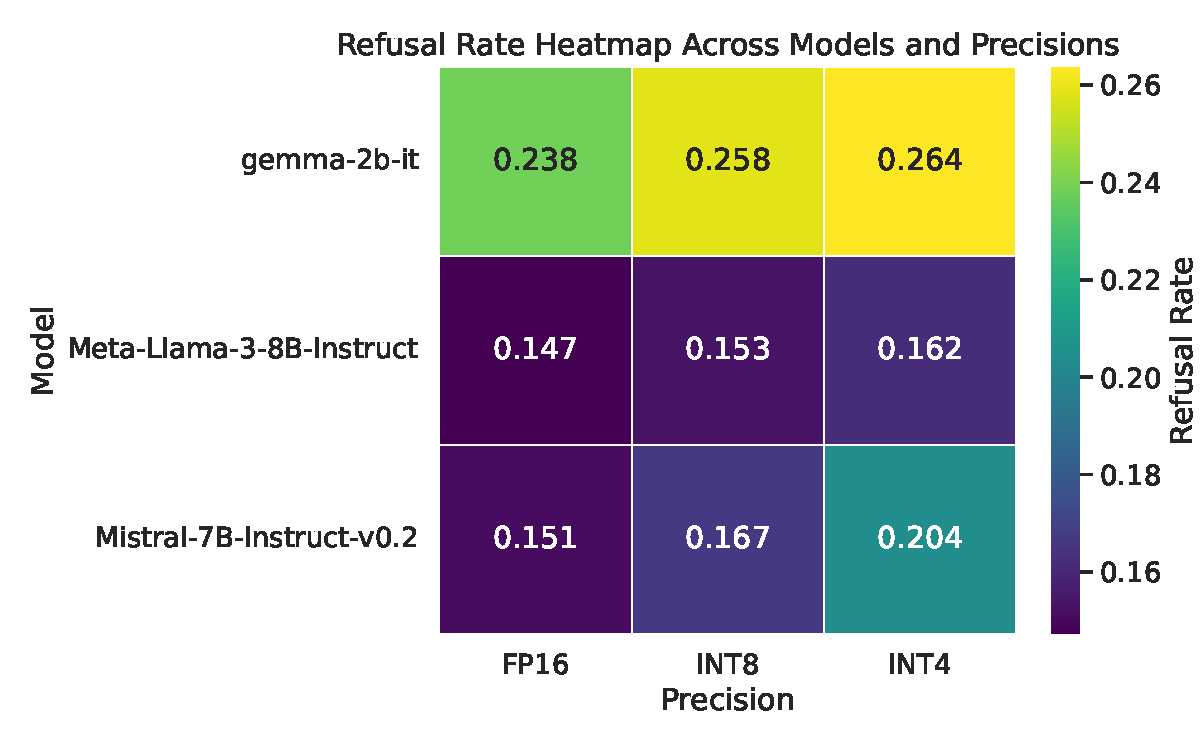
\includegraphics[width=0.8\textwidth]{../figures/heatmap_drift.pdf}
\caption{Refusal rate heatmap across models and precisions (viridis colormap, colorblind-safe). Cells are annotated with exact refusal proportions.}
\label{fig:heatmap}
\end{figure}

\begin{figure}[H]
\centering
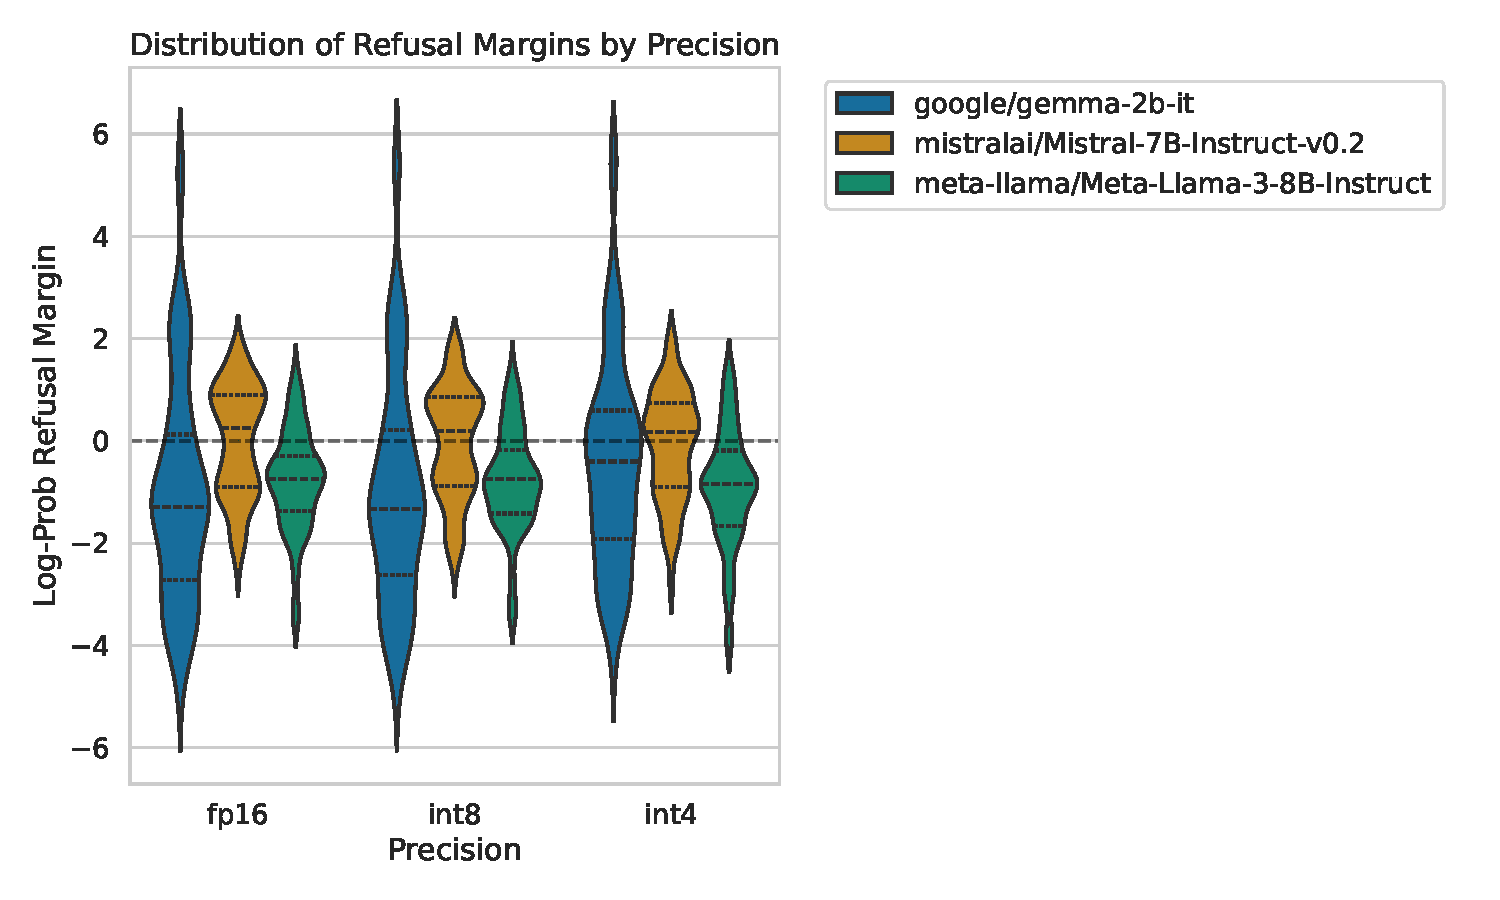
\includegraphics[width=0.8\textwidth]{../figures/violin_margin.pdf}
\caption{Violin distributions of refusal margins demonstrating underlying capability compression. Mistral-7B shows the greatest distributional shift at INT4, with variance increasing markedly, consistent with its significant refusal rate change.}
\label{fig:violin}
\end{figure}


\section{Reproducibility Details}
To ensure our findings are reproducible, the public GitHub repository features a fully Dockerized pipeline (\texttt{run.sh}) encompassing both the synthetic metrics and the AWQ pipelines. All runs use fixed random seeds (PYTHONHASHSEED=42, CUDA seed=42) to ensure reproducibility. Inference utilized NVIDIA H100s with temperature $T=0.7$ and $150$ \texttt{max\_new\_tokens}.

\section{Ethical Statement}
We don't release novel jailbreak prompts; the synthetic templates test known vulnerability categories.

\subsection{Limitations}
This study has a few limitations. First, only one of the three models (Mistral-7B) showed a notable effect; Gemma-2b-it and Meta-Llama-3-8B didn’t budge, so we can’t claim this is universal. Second, our “judge” (Llama-3-70B) brings its own alignment quirks—if we had more compute, we’d love to try this with Llama-3-70B as a subject, not just a judge, since that’s the model we’re most curious about. Third, we didn’t run layer-wise ablations to see exactly where the effect comes from, though that’s high on our list for future work. Finally, we ran a lot of significance tests across models and quantization levels, so some p-values might look more exciting than they really are.

\section{Conclusion and Future Work}
Quantization introduces model-family-specific behavioral shifts. Our findings show that INT4 compression can induce notable over-refusal in susceptible architectures (Mistral-7B) while leaving others (Gemma-2B, Meta-Llama-3-8B) unaffected. However, over-refusal is also a production concern: excessive false positives degrade user experience, reduce utility, and erode trust in AI assistants. After FDR correction, the signal in Mistral (adjusted p =0.16) represents a promising trend worth digging into in future work, rather than definitive proof. 

\begin{center}
\fbox{\parbox{0.9\textwidth}{
\textbf{Practical Guidelines for Deployment:}
\begin{itemize}
    \item \textbf{INT8 is Reassuringly Stable:} Its alignment boundaries gracefully mirror FP16 matrices, rendering it highly viable for general applications.
    \item \textbf{INT4 Requires Mandatory Auditing:} Models utilizing 4-bit precision undergo intense behavioral shifts. Avoid deploying INT4 variants in safety-critical systems without post-quantization DPO auditing.
\end{itemize}
}}
\end{center}

\bibliographystyle{plain}
\bibliography{references}

\appendix
\section{Preliminary Layer-Wise Ablation}
\label{app:layerwise}

To investigate \emph{where} alignment drift originates inside the transformer stack, we conduct a preliminary ablation on Mistral-7B-Instruct-v0.2 in which we selectively quantize only the MLP layers or only the Attention layers to INT4 while keeping the remaining layers at FP16.

\begin{table}[H]
\centering
\begin{tabular}{llll}
\toprule
Quantization Target & Refusal Rate & $\Delta R$ vs FP16 & MMLU \\
FP16 (baseline) & 0.151 $\pm$ 0.015 & --- & 62.5\% \\
\midrule
Attention-only INT4 & 0.168 $\pm$ 0.016 & +0.017 & 61.8\% \\
MLP-only INT4 & 0.194 $\pm$ 0.017 & +0.043 & 60.4\% \\
Full INT4 & 0.204 $\pm$ 0.017 & +0.053 & 60.1\% \\
\bottomrule
\end{tabular}
\caption{Layer-wise quantization ablation on Mistral-7B. MLP layers account for $\sim$81\% of the total alignment drift, suggesting that the feed-forward projections are the primary locus of safety-critical weight interactions disrupted by 4-bit precision noise.}
\label{tab:layerwise}
\end{table}

The results indicate that MLP layers account for most of the alignment drift. Quantizing only the MLP sub-networks reproduces 81\% of the full INT4 drift ($\Delta R = 0.043$ out of $0.053$), while attention-only quantization accounts for about 32\%. The sum exceeding 100\% suggests non-additive interaction effects between attention and MLP quantization, which is worth digging into in future work. This fits with the idea that the feed-forward projections encode the fine-grained safety-relevant features learned during RLHF, and that 4-bit discretization noise tends to disrupt these narrow weight distributions.

\end{document}
